\chapter{序論}

\section{目的}

マグネシウム(Mg)は実用金属中において最も軽量であるが,耐食性が悪く, 発火しやすいという欠点がある.LPSO ( Long Period Stacking Order ) 構造をもった Mg は比降伏強度で超々ジュラルミンの 1.2 倍の特性を持ち, かつ難燃性であるため次世代の航空機の構造材料として国内外から注目を集めている\cite{Th}. LPSO 構造は, 母相 hcp 構造の [0001] 方向に対して周期的に積層欠陥が導入されることで長周期性を有する構造である.

西谷研究室では, この LPSO 構造の生成機構として「積層欠陥部に L1$_2$ クラスターが形成され, そこから排斥された Zn, Y が, 濃化して新たな L1$_2$ クラスターを形成する」というシナリオを立てた. このシナリオの実現性について, 第一原理計算を用いて評価してきた. 第一原理計算は, 量子力学を支配するシュレディンガー方程式を精確に解いて, 原子の種類だけから電子構造を求め, いろいろな物性を予測する計算である. 計算の結果, 系全体のエネルギーは溶質原子と L1$_2$ クラスターとの距離が離れるにつれ単調に減少し安定となった. しかしそれは中周期的に溶質原子が濃化するという LPSO の構造から予想される結果に反するものであった.

そこで,いままで検証してきた溶質原子ではなく,違う構造物としてSmall Clusterに注目した.
Small Clusterは清原らが見出した比較的安定な構造であり,これと L1$_2$ クラスターの相互作用を
求めた\cite{kiyohara}.また,このSmall Clusterの移動機構を解明するために,一般的な拡散機構で重要となる
空孔がどの位置で安定であるかを検討した.これらのエネルギー計算には第一原理計算ソフト
VASPを求めた\cite{vasp}.

\section{材料構造の基礎的知識}
ここでは,本研究を遂行するにあたって必要となった材料の構造に関する基礎的知識を
まとめて記述する.「LPSO構造」およびそれを構成する基本単位である「積層欠陥」,および「空孔拡散」と「クラスター拡散」である.これらは,材料分野においては一般的な知識であるが,計算モデル,結果を
理解する上で不可欠と考えて最初にまとめて示しておく.

\subsection{積層欠陥}
積層欠陥とは積層順序の連続性が局所的に乱れた欠陥である. 図\ref{fig1}に hcp 構造の積層欠陥の様子を表した模式図を示した. hcp 構造ではこの図で示すように [0001] 方向に最密面が ABAB と積層しており, 赤枠で囲った原子を赤矢印の方向にずらすと, 積層順序が ABCA となる. その際に赤の破線で示した部分が積層欠陥面となる. そして hcp 構造上に発生した積層欠陥面の上下の黄丸で示した層を中心とした積層順序を考えると, それぞれ ABC,BCA となっている. このことから hcp 構造において積層欠陥が発生すると cubic 構造である fcc 構造が導入されることがわかる.

\begin{figure}[htbp]
	\begin{center}
		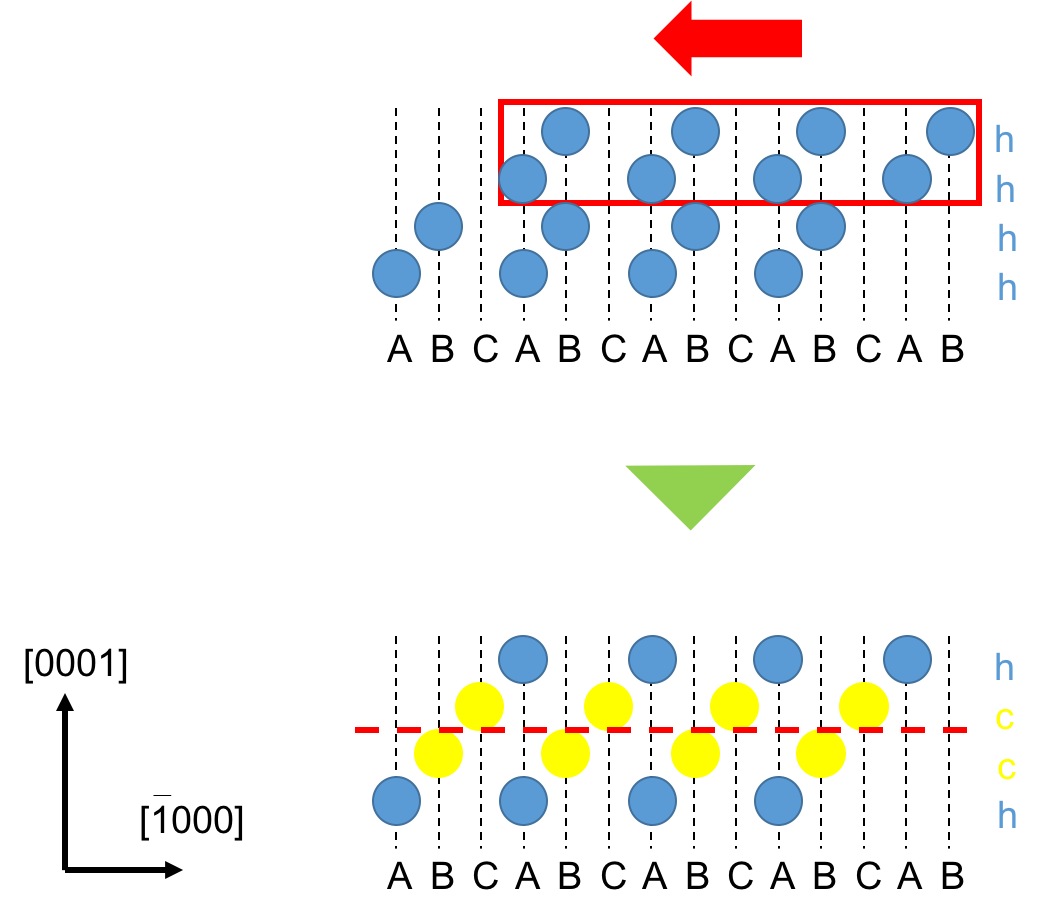
\includegraphics[width=100mm]{../intro/stuc.png}
		\caption{hcp 構造の積層欠陥の様子を表した模式図. 青丸は hexgonal 構造, 黄丸は cubic 構造を示している. また赤の破線部は積層欠陥部を示している.}
		\label{fig1}
	\end{center}
\end{figure}

\subsection{LPSO 構造}
LPSO ( Long Period Stacking Order ) 構造はその名称が示す通り,長周期の積層欠陥を含んだ構造であり,その積層欠陥部に溶質原子が濃化していることが研究の初期に判明していた. しかし, 液相から直接生成する合金系や, 固相から時効析出によって生成する系など多くの系で微妙に異なる構造を示すことが報告された. LPSO-Mg では下記の特徴がある.

\begin{itemize}
  \item $[0001]$ 方向において中周期的に積層欠陥が導入されている.
  \item 積層欠陥部には溶質原子であるZn,Yが集まっている.
  \item 集まった溶質原子が積層欠陥部において L1$_2$ クラスターを形成している.
\end{itemize}

\subsection{空孔拡散}
結晶中には原子の存在しない格子点があり, これを空孔(vacancy)という. 空孔と隣接する原子が位置を交換することにより拡散が起こる.
完全なカバレッジに近づく高いカバレッジレベルでの表面拡散の主な方法として起こり得る. このプロセスは、スライディングパズルで周りを滑るような方法に似ている. 高い拡散速度と低い空孔濃度のために、空孔拡散を直接観察することは非常に困難である. また, 単空孔と複空孔の拡散の模式図を図\ref{fig2}, 図\ref{fig3}に示した. 単空孔よりも複空孔の方が拡散の可能性が高くなる. それは図\ref{fig2}において赤線の山で表現している activation barrier 単空孔のほうが高いのが原因である.

\begin{figure}[htbp]
	\begin{center}
		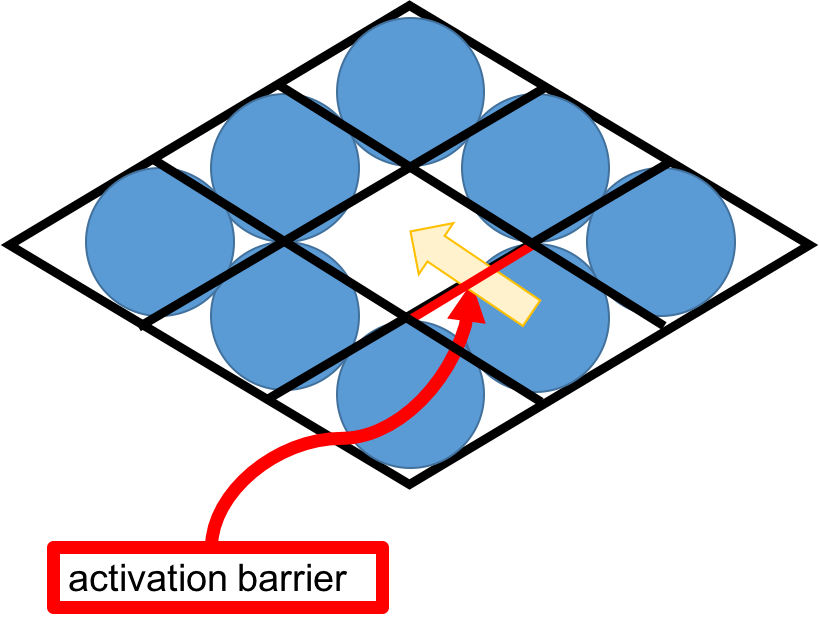
\includegraphics[width=80mm]{../intro/monovacancy.png}
        \caption{単空孔の拡散の模式図.}
		\label{fig2}
	\end{center}
\end{figure}

\begin{figure}[htbp]
	\begin{center}
		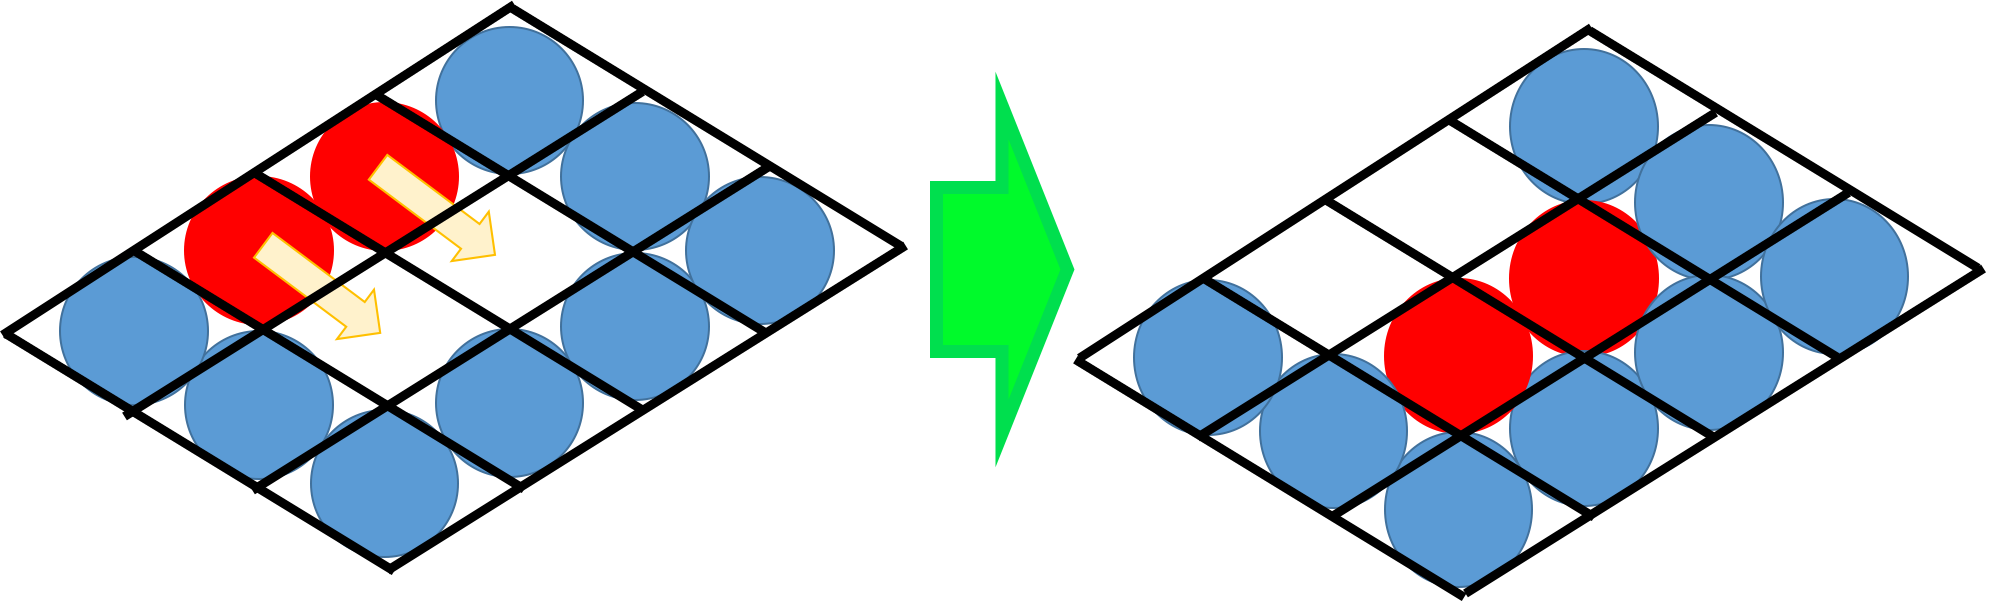
\includegraphics[width=130mm]{../intro/divacancy.png}
        \caption{複空孔の拡散の模式図.}
		\label{fig3}
	\end{center}
\end{figure}


\subsection{クラスター拡散}
クラスター拡散とは複数の原子の塊の移動のことを言う. クラスターの動きは、個々の原子, クラスターのセクション, またはクラスター全体が移動する場合がある.
クラスター拡散に関して, 結晶の表面では可能であるが, バルクでは不可能である.
理由は図\ref{fig4}で示すように表面では上層がないため動くことが可能だが, 図\ref{fig5}のようなバルクでは上層も原子が詰まっており動くことができないからである.

\begin{figure}[htbp]
	\begin{center}
		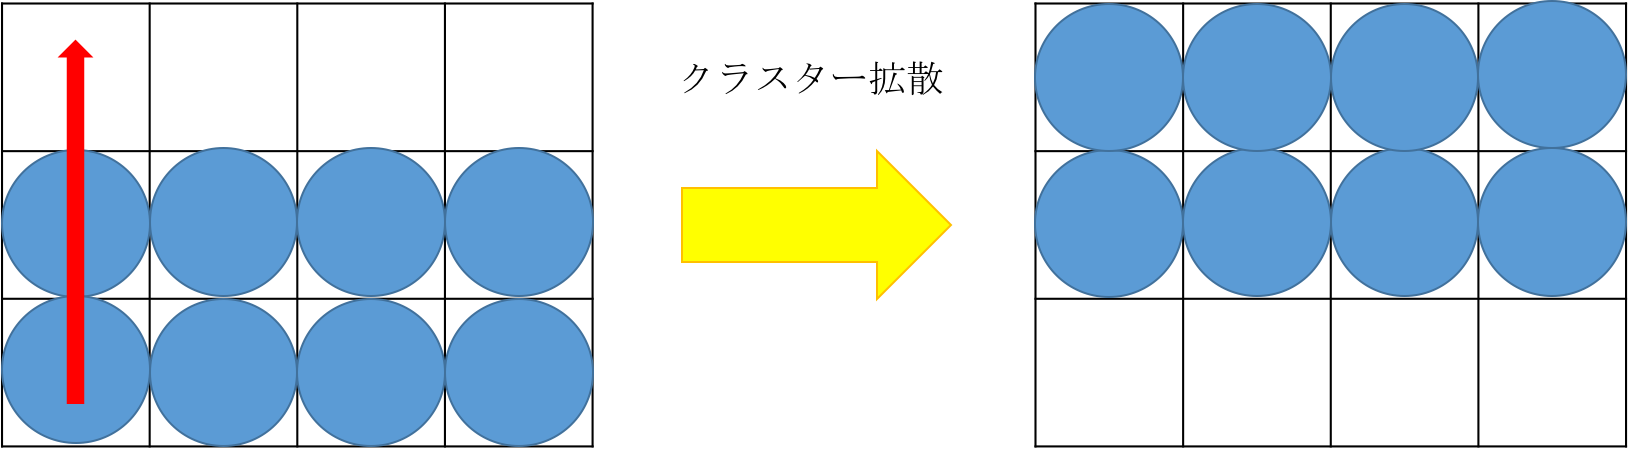
\includegraphics[width=100mm]{../intro/kakusan.png}
		\caption{クラスター拡散の模式図.}
		\label{fig4}
	\end{center}
\end{figure}

\begin{figure}[htbp]
	\begin{center}
		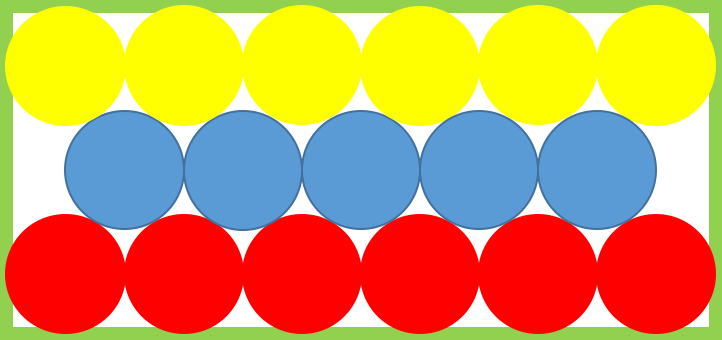
\includegraphics[width=70mm]{../intro/balc.png}
        \caption{バルク内の模式図.}
		\label{fig5}
	\end{center}
\end{figure}
